\documentclass[10pt,oneside, a4paper]{article}
\usepackage[utf8]{inputenc}
\usepackage{mathtools}
\usepackage{array}
\usepackage[italian]{babel}
\usepackage[pdfusetitle]{hyperref}
\usepackage{cancel}
\usepackage{xcolor}
\usepackage[pdftex]{graphicx}
%\usepackage{caption}
\usepackage{titling}
%\usepackage{comment}
\usepackage{tabularx}
\usepackage[top=2cm, bottom=2cm, left=1cm, right=1cm]{geometry}
\usepackage{subfiles}

\title{Il formulario bellino}
\author{Lorenzo Cauli}

\setlength{\footskip}{90pt}
\setlength{\droptitle}{-10em}
\graphicspath{./images/}

\DeclareMathOperator{\arccot}{arccot}

\begin{document}
    \maketitle
    {\centering 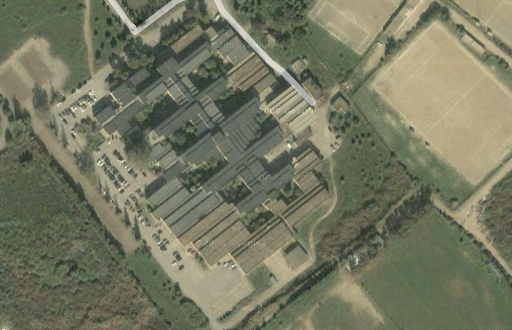
\includegraphics[width=400pt]{images/scano.png} \par}
    \newpage
    \tableofcontents

    \newpage
    \section{Derivate}
    \subfile{include/derivate/01_razionali}
    \subfile{include/derivate/02_irrazionali}
    \newpage
    \subfile{include/derivate/03_esponenziali}
    \subfile{include/derivate/04_logaritmiche}
    \subfile{include/derivate/05_goniometriche}
    \subfile{include/derivate/06_operazioni}

    \newpage
    \section{Integrali}
    \subsection{AAAA}
    \huge{WIP}

\end{document} 